% Template for PLoS
% Version 3.1 February 2015
%
% To compile to pdf, run:
% latex plos.template
% bibtex plos.template
% latex plos.template
% latex plos.template
% dvipdf plos.template
%
% % % % % % % % % % % % % % % % % % % % % %
%
% -- IMPORTANT NOTE
%
% This template contains comments intended 
% to minimize problems and delays during our production 
% process. Please follow the template instructions
% whenever possible.
%
% % % % % % % % % % % % % % % % % % % % % % % 
%
% Once your paper is accepted for publication, 
% PLEASE REMOVE ALL TRACKED CHANGES in this file and leave only
% the final text of your manuscript.
%
% There are no restrictions on package use within the LaTeX files except that 
% no packages listed in the template may be deleted.
%
% Please do not include colors or graphics in the text.
%
% Please do not create a heading level below \subsection. For 3rd level headings, use \paragraph{}.
%
% % % % % % % % % % % % % % % % % % % % % % %
%
% -- FIGURES AND TABLES
%
% Please include tables/figure captions directly after the paragraph where they are first cited in the text.
%
% DO NOT INCLUDE GRAPHICS IN YOUR MANUSCRIPT
% - Figures should be uploaded separately from your manuscript file. 
% - Figures generated using LaTeX should be extracted and removed from the PDF before submission. 
% - Figures containing multiple panels/subfigures must be combined into one image file before submission.
% For figure citations, please use "Fig." instead of "Figure".
% See http://www.plosone.org/static/figureGuidelines for PLOS figure guidelines.
%
% Tables should be cell-based and may not contain:
% - tabs/spacing/line breaks within cells to alter layout or alignment
% - vertically-merged cells (no tabular environments within tabular environments, do not use \multirow)
% - colors, shading, or graphic objects
% See http://www.plosone.org/static/figureGuidelines#tables for table guidelines.
%
% For tables that exceed the width of the text column, use the adjustwidth environment as illustrated in the example table in text below.
%
% % % % % % % % % % % % % % % % % % % % % % % %
%
% -- EQUATIONS, MATH SYMBOLS, SUBSCRIPTS, AND SUPERSCRIPTS
%
% IMPORTANT
% Below are a few tips to help format your equations and other special characters according to our specifications. For more tips to help reduce the possibility of formatting errors during conversion, please see our LaTeX guidelines at http://www.plosone.org/static/latexGuidelines
%
% Please be sure to include all portions of an equation in the math environment.
%
% Do not include text that is not math in the math environment. For example, CO2 will be CO\textsubscript{2}.
%
% Please add line breaks to long display equations when possible in order to fit size of the column. 
%
% For inline equations, please do not include punctuation (commas, etc) within the math environment unless this is part of the equation.
%
% % % % % % % % % % % % % % % % % % % % % % % % 
%
% Please contact latex@plos.org with any questions.
%
% % % % % % % % % % % % % % % % % % % % % % % %

\documentclass[10pt,letterpaper]{article}
\usepackage[top=0.85in,left=2.75in,footskip=0.75in]{geometry}

% Use adjustwidth environment to exceed column width (see example table in text)
\usepackage{changepage}

% Use Unicode characters when possible
\usepackage[utf8]{inputenc}

% textcomp package and marvosym package for additional characters
\usepackage{textcomp,marvosym}

% fixltx2e package for \textsubscript
\usepackage{fixltx2e}

% amsmath and amssymb packages, useful for mathematical formulas and symbols
\usepackage{amsmath,amssymb}

% cite package, to clean up citations in the main text. Do not remove.
\usepackage{cite}

% Use nameref to cite supporting information files (see Supporting Information section for more info)
\usepackage{nameref,hyperref}

% line numbers
\usepackage[right]{lineno}

% ligatures disabled
\usepackage{microtype}
\DisableLigatures[f]{encoding = *, family = * }

% rotating package for sideways tables
\usepackage{rotating}

\usepackage{verbatim}   % useful for program listings

% Remove comment for double spacing
%\usepackage{setspace} 
%\doublespacing

% Text layout
\raggedright
\setlength{\parindent}{0.5cm}
\textwidth 5.25in 
\textheight 8.75in

% Bold the 'Figure #' in the caption and separate it from the title/caption with a period
% Captions will be left justified
\usepackage[aboveskip=1pt,labelfont=bf,labelsep=period,justification=raggedright,singlelinecheck=off]{caption}

% Use the PLoS provided BiBTeX style
% \bibliographystyle{plos2015}
\bibliographystyle{apalike}

% Remove brackets from numbering in List of References
\makeatletter
\renewcommand{\@biblabel}[1]{\quad#1.}
\makeatother

% Leave date blank
\date{}

% Header and Footer with logo
\usepackage{lastpage,fancyhdr,graphicx}
\usepackage{epstopdf}
\pagestyle{myheadings}
\pagestyle{fancy}
\fancyhf{}
\lhead{
\includegraphics[width=2.0in]{PLOS-submission.eps}}
\rfoot{\thepage/\pageref{LastPage}}
\renewcommand{\footrule}{\hrule height 2pt \vspace{2mm}}
\fancyheadoffset[L]{2.25in}
\fancyfootoffset[L]{2.25in}
\lfoot{\sf PLOS}

%% Include all macros below

\newcommand{\lorem}{{\bf LOREM}}
\newcommand{\ipsum}{{\bf IPSUM}}

%% END MACROS SECTION


\begin{document}
\vspace*{0.35in}

% Title must be 250 characters or less.
% Please capitalize all terms in the title except conjunctions, prepositions, and articles.
\begin{flushleft}
{\Large
\textbf\newline{Filament Recycling and Sustained Contractile Flows in an Actomyosin Cortex}
}
\newline
% Insert author names, affiliations and corresponding author email (do not include titles, positions, or degrees).
\\
William McFadden\textsuperscript{1},
Patrick McCall\textsuperscript{2},
Edwin Munro\textsuperscript{3,*}
\\
\bigskip
\bf{1} Biophysical Sciences Program, University of Chicago, Chicago, IL, USA
\\
\bf{2} Department of Physics, University of Chicago, Chicago, IL, USA
\\
\bf{3} Department of Molecular Genetics and Cell Biology, University of Chicago, Chicago, IL, USA
\\
\bigskip

% Insert additional author notes using the symbols described below. Insert symbol callouts after author names as necessary.
% 
% Remove or comment out the author notes below if they aren't used.
%
% Primary Equal Contribution Note
%\Yinyang These authors contributed equally to this work.

% Additional Equal Contribution Note
% Also use this double-dagger symbol for special authorship notes, such as senior authorship.
%\ddag These authors also contributed equally to this work.

% Current address notes
%\textcurrency a Insert current address of first author with an address update
% \textcurrency b Insert current address of second author with an address update
% \textcurrency c Insert current address of third author with an address update

% Deceased author note
%\dag Deceased

% Group/Consortium Author Note
%\textpilcrow Membership list can be found in the Acknowledgments section.

% Use the asterisk to denote corresponding authorship and provide email address in note below.
* emunro@uchicago.edu

\end{flushleft}
% Please keep the abstract below 300 words
\section*{Abstract}
Fill in abstract later.


% Please keep the Author Summary between 150 and 200 words
% Use first person. PLOS ONE authors please skip this step. 
% Author Summary not valid for PLOS ONE submissions.   
\section*{Author Summary}
In this paper, we develop and analyze a minimal model for 2D active networks based on the cortical cytoskeleton of eukaryotic embryos.  Our model introduces a series of coarse-grained approximations for simultaneous comparison of cross-link stress dissipation, myosin driven active stress generation and a form of rapid filament turnover we term {\em filament recycling}.  We generate computational simulations based on the model and demonstrate that our minimal assumptions are sufficient to drive network contraction and to set up steady state flow profiles such as those found in the cortex of developing embryos and migrating cells.  Our analysis sheds insight on potential microscopic control parameters governing broad qualitative differences in 2D active networks. 
\linenumbers

\section*{Introduction}

\paragraph{}  Cortical flow is a fundamental and ubiquitous form of cellular deformation that underlies cell polarization, cell division, cell crawling and multicellular tissue morphogenesis\cite{cellmech_flows3,cellmech_flows2}.  These flows arise within the actomyosin cortex, a thin layer of cross-linked actin filaments and myosin motors that lies just beneath the plasma membrane \cite{Salbreux2012536}. The active forces that drive cortical flows are thought to be generated by myosin motors pulling against individual actin filaments \cite{Munro2004413}. These forces must be integrated within cross-linked networks to build macroscopic contractile stress.  At the same time, cross-linked networks resist deformation and this resistance must be dissipated by network remodeling to allow macroscopic network deformation and flow.  How force production and dissipation depend on motor activity, network architecture and remodeling remains poorly understood.

Current models for cortical flow rely on coarse-grained descriptions of actomyosin networks as active fluids, whose motions are driven by gradients of active contractile stress and opposed by an effectively viscous resistance\cite{cellmech_flows}.  In these models, gradients of active stress are assumed to reflect spatial variation in motor activity and viscous resistance is assumed to reflect the internal dissipation of elastic resistance due to local remodeling of filaments and/or cross-links \cite{PhysRevLett.106.028103}.  A key virtue of these models is that their behavior is governed by a few parameters (active stress and effective viscosity).  By coupling an active fluid description to simple kinetic models for network assembly and disassembly and making active stress and effective viscosity depend on e.g network density and turnover rates, it is possible to capture phenomenological descriptions of cortical flow.  Models based on this active fluids description can successfully reproduce spatiotemporal dynamics of cortical flow observed during polarization \cite{cellmech_flows}, cell division \cite{Turlier2014114,PhysRevLett.103.058102}, cell motility \cite{Keren:2009aa,RevModPhys.85.1143} and tissue morphogenesis \cite{Heisenberg2013948}.  

However, to understand how cells exert physiological control over cortical deformation and flow, or to build and tune networks with desired properties {\em in vitro}, it is essential to connect this coarse-grained description to the microscopic origins of force generation and dissipation within cross-linked actomyosin networks.  Both active stress and effective viscosity depend sensitively on microscopic parameters including densities of filaments, motors and cross-links, force-dependent motor/filament interactions, cross-link dynamics and network turnover rates.  Thus a key challenge is to understand how tuning these microscopic parameters controls the dynamic interplay between active force generation and passive relaxation to control macroscopic dynamics of cortical flow.

\paragraph{} Studies in living cells have documented fluid-like stress relaxation on timescales of 10-100s of seconds \cite{cellmech_flows,cellmech_flows2,cellmech_flows3,rheo_fluid,rheo_fluid2,cell_rheo_exp}.  These modes of stress relaxation are thought to arise both from the transient binding/unbinding of individual cross-links and from the turnover (assembly/disassembly) of actin filaments (ref).  Studies of cross-linked and/or bundled actin networks {\em in vitro} suggest that cross-link unbinding may be sufficient to support viscous relaxation (creep) on very long timescales\cite{rheo_crosslinksmatter,rheo_crosslinkslip1,rheo_crosslinkslip2,rheo_crosslinkslip3,rheo_nonaffine}, but is unlikely to explain the rapid large scale cortical deformation and flow observed in living cells.  It has been proposed in the field that rapid actin turnover must play a significant role as well. Indeed, photokinetic and single molecule imaging studies studies reveal rapid turnover of cortical actin filaments in living cells on timescales of 10-100 seconds \cite{Robin:2014aa}. Previous theoretical models have explored  the dependence of stress relaxation on cross-link binding and unbinding analytically \cite{theo_crosslinkslip1,theo_crosslinkslip2} and others have explicitly modeled reversible cross-linking in combination with complex mechanics of filament bundles \cite{model_taeyoon,rheo_crosslinkslip2,theo_crosslinkslip3}.  However, until very recently \cite{Mak:2016aa} very little attention has been paid to actin turnover as mechanism of stress relaxation. 

Recent work has also begun to reveal insights into mechanisms that govern active stress generation in disordered actomyosin networks. In vitro studies have confirmed that local interactions among actin filaments and myosin motors are sufficient to drive macroscopic contraction of disordered networks \cite{rheo_2D1}.  Theoretical studies suggest that asymmetrical compliance of actin filaments (stiffer under extension than compression) and spatial differences (dispersion) in motor activity are sufficient conditions for contraction in one \cite{1367-2630-14-3-033037} and two \cite{PhysRevX.4.041002} dimensional networks, although other routes to contractility may also exist \cite{PhysRevX.4.041002}.  Further work has explored how modulation of network architecture, cross-link dynamics and motor density, activity and assembly state can shape rates and patterns of network deformation \cite{10.1371/journal.pone.0039869,Alvarado:2013aa,C0SM00494D} or network rheology \cite{0295-5075-85-1-18007,rheo_active}.  

Significantly, {\em in vitro} models for disordered actomyosin networks have used stable actin filaments, and these networks support only transient contraction, either because of network collapse\cite{Alvarado:2013aa}, or buildup of elastic resistance (ref? I don't know about this one), or because network rearrangements (polarity sorting) dissipate the potential to generate contractile force \cite{Ndlec:1997aa,Surrey1167}. This suggest that continuous turnover of actin filaments may play a key role in allowing sustained deformation and flow. Recent theoretical and modeling studies have begun to explore how this could work \cite{2015arXiv150706182H,Mak:2016aa,10.1371/journal.pone.0000696}, and to explore dynamic behaviors that can emerge in contractile material with turnover \cite{PhysRevLett.113.148102}. However, there is much to learn about how the buildup and maintenance of contractile force during continuous deformation and flow depends local interplay of network architecture, motor activity and filament turnover.



\paragraph{}  The goal of this work was to build a computational bridge between the microscopic description of cross-linked actomyosin networks and the coarse grained macroscopic description of an active fluid.  We sought to capture the essential microscope features (dynamic cross-links, active motors and semi flexible actin filaments with asymmetric compliance and continuous filament recycling), but in a way that is sufficiently simple to allow systematic exploration of how parameters that govern network deformation and flow in an active fluid theory depend on microscopic parameters. To this end, we introduce several coarse-grained approximations into our representation of filament networks. First, we represent semi-flexible actin filaments as chains of simple springs with asymmetric compliance (stronger in extension than compression). Second, we replace  dynamic binding/unbinding of elastic cross-links with a coarse-grained representation in terms of molecular friction \cite{theo_friction,theo_frictionSam,theo_molefric}, such that filaments can slide past each other against a constant fictional resistance. Third, we used a similar scheme to introduce active motors at filament crossover points with a simple linear force/velocity relationship, and we introduce dispersion of motor activity by making only a subset of filament overlaps active \cite{theo_frictionShila}.  Finally, we model filament turnover by regularly reseting a subset of filaments to a new unstrained position. Importantly, these simplification allows us to extend our single polymer models to dynamical systems of larger network models for direct comparison between theory and modeling results. This level of coarse graining will therefore make it easier to understand classes of behavior for varying compositions of cross-linked filament networks. In addition, it allows us to compute a new class of numerical simulations efficiently, which gives us concrete predictions for behaviors in widely different networks with measurable dependencies on molecular details. 
  

% You may title this section "Methods" or "Models". 
% "Models" is not a valid title for PLoS ONE authors. However, PLoS ONE
% authors may use "Analysis" 
\section*{Models}

\begin{figure}[h!]
\centering
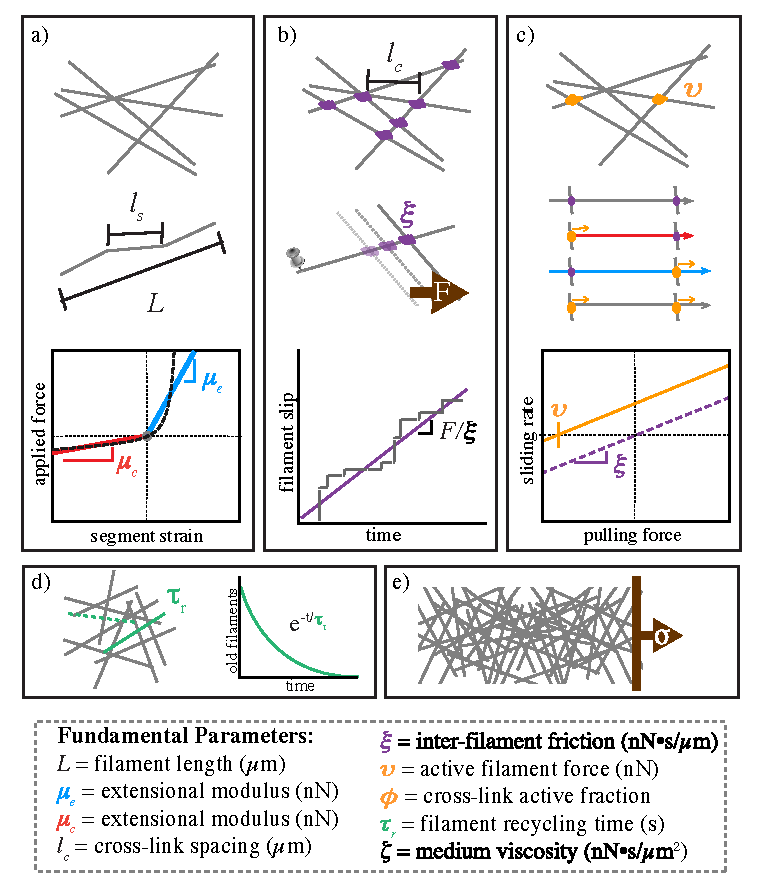
\includegraphics[width=\hsize]{figures/fig2/fig2}
\caption{\label{fig:sim} Schematic of modeling framework. a) Asymmetric filament compliance.Filaments have smaller spring constant for compression than for extension. b) Cross-link slip. Cross-links are coupled by an effective drag, such that their relative motion is
proportional to any applied force. c) Motor activity. Filament activity manifests as a basal sliding rate even in the absence of an external force. Fractional activity. Only a subset of filament cross-links are active, resulting in differential force exertion along the filament. d) Filament recycling. Filaments are turned over at a constant rate, leading to a refreshing in the strain state of all filaments after a characteristic timescale. e) Applied stress. In simulations with passive cross-links, and external stress is applied as force filed acting on a fixed spatial domain.}
\end{figure}

Our goal was to model essential microscope features of cross-linked actomyosin networks (semi flexible actin filaments with asymmetric compliance, dynamic cross-links, active motors and and continuous filament recycling), in a way that is simple enough to allow systematic exploration of how tuning these microscopic features controls macroscopic network deformation and flow. We focus on 2D networks for computational tractability and because they capture a reasonable approximation of the quasi-2D cortical actomyosin networks that govern flow and deformation in many eukaryotic cells\cite{cellmech_flows}, or the quasi-2D networks used in recent in vitro studies\cite{rheo_2D1,rheo_2D2}.


\subsection*{Asymmetric filament compliance}
We model individual filaments as chains of springs with relaxed length $l_s$.  Filaments can therefore be represented as a sequence of nodes with positions $\mathbf{x_i}$ and nearest neighbor force interactions, $\mathbf{F^{\mu}_i}$, of the form

\begin{equation}
\label{eqn:spring}
|F^{\mu}_i| = \mu\cdot\frac{|\mathbf{x_{i+1}}-\mathbf{x_i}|-l_s}{l_s} +\mu\cdot\frac{|\mathbf{x_{i-1}}-\mathbf{x_i}|-l_s}{l_s}
\end{equation}





where the modulus, $\mu$, is a composite quantity representing both filament and cross-linker compliance in a manner similar to a proposed effective medium theory \cite{theo_crosslinknonlinear}.   To model asymmetric filament compliance, we assign the modulus $\mu$, a different value depending on whether $|\mathbf{x_{i-1}}-\mathbf{x_i}|-l_s$ (the strain) is greater or less than 0. In the limit of highly rigid cross-links and flexible filaments, our model reduces to the pure semi-flexible filament models of \cite{theo_hlm,theo_hlm2}.  In the opposite regime of nearly rigid filaments and highly flexible cross links, our method is still largely similar to the model of \cite{theo_crosslinknonlinear} in small strain regimes before any nonlinear cross link stiffening.  In a departure from those models, we assume here that the magnitude of the force on interior cross-links is the same as those on the exterior.  This approach ignores the variation in strain on these two sets of cross-links as addressed in \cite{theo_crosslinknonlinear}, but we choose to ignore this variation in favor of an approximated, global mean approach.  



\subsection*{Drag-like coupling between overlapping filaments}
\label{exp_drag}
Previous models represent cross-linkers as elastic connections between pairs of points on neighboring filaments that appear and disappear with either fixed or strain-dependent probabilities \cite{model_taeyoon,theo_crosslinknonlinear}.  Here, we introduce a simpler coarse-grained model for dynamic cross-links by replacing many transient elastic interactions with an effective drag-like coupling between every pair of overlapping segments.
\begin{equation}
\label{eqn:drag}
\mathbf{F^{\xi}_i} = \xi \cdot \int^{s_{i+1}}_{s_{i-1}} ds \frac{l_s-|s-s_i|}{l_s} \: (\mathbf{v_i}-\mathbf{v_j}) \: p_{ij}(s)
\end{equation}

Where $p_{ij}(s)$ represents the locational distribution of cross-link points (equal to 1 at locations of cross-links and 0 elsewhere) and $\mathbf{v_i}$ and $\mathbf{v_j}$ represent the velocities of the $i$th and $j$th filament segment.  This model assumes a linear relation between applied force and the velocity difference between attached segments.  This drag-like coupling has been shown to be an adequate approximation in the case of ionic cross-linking of actin\cite{mol_fric,theo_hydroish2}, and can be found in the theoretical basis of force-velocity curves for myosin bound filaments\cite{theo_frictionShila}. Although non-linearities can arise through force dependent detachment kinetics and/or non-linear force extension of cross-links, we assume that inhomogeneities from non-linear effects are of second or higher order. With this assumption, the motion of filaments can be described by a dynamical equation of the form

\begin{equation}
\label{eqn:syst1}
L\zeta\mathbf{ v_i} +\mathbf{F^{\xi}_i}= \mathbf{F^{\mu}_i}
\end{equation}

Here, the first term in the integral is the filament's intrinsic drag through its embedding fluid, $\zeta$, while the second comes from the drag-like coupling between filaments, $\xi$.  

\subsection*{Active coupling for motor driven filament interactions}

To add motor activity we select a subset of cross-linked points and impart an additional force of magnitude $\upsilon$ directed in the orientations of the individual filaments, $\mathbf{u_i}$.  This leads to a modification of the equation of motion to

\begin{equation}
\label{eqn:moto}
\mathbf{F^{\upsilon}_i}= \mathbf{\hat{u}_i}\cdot\upsilon\int ds \sum _j \:  \frac{l_s-|s-s_i|}{l_s} p_{ij}q_{ij}
\end{equation}

In this formulation, only at the subset of points where  $p_{ij}=1$ and $q_{ij}=1$ will there be a force imparted.  In our simulations we let $q_{ij}$ be selected randomly such that $\bar{q}=\phi$, where $\bar{q}$ indicates the mean of $q$.

Finally, for each active force, $\mathbf{F^{\upsilon}_j}$, imparted by filament $j$, we must also impart the opposite force onto the filament $i$ as well.  Therefore, the entire force balance equation with activity will appear as

\begin{equation}
\label{eqn:syst3}
L\zeta\mathbf{ v_i} +\mathbf{F^{\xi}_i}= \mathbf{F^{\mu}_i}+\mathbf{F^{\upsilon}_i} - \sum_{j}\mathbf{F^{\upsilon}_j}p_{ij}q_{ij}
\end{equation}

\subsection*{2D network formation}

We used a mikado model approach \cite{Unterberger2014} to initialize a minimal network of connected unstressed linear filaments in a rectangular 2D domain. We generate 2D networks of these semi-flexible filaments by laying down straight lines of length, L, with random position and orientation. We then assume that overlapping filaments become cross-linked at their points of overlap. Although real cytoskeletal networks may form with non-negligible anisotropy, for simplicity, we focus on isotropically initialized networks. We define the density using the average distance between cross-links along a filament, $l_c$. A simple geometrical argument can then be used to derive the number of filaments filling a domain as a function of $L$ and $l_c$\cite{theo_hlm}.  Here, we use the approximation that the number of filaments needed to tile a rectangular domain of size $W \times H$  is $2WH/Ll_c$, and that the length density is therefore simply, $1/l_c$. In the absence of cross-link slip, we expect the network to form a connected solid with a well defined elastic modulus\cite{theo_hlm,theo_hlm2}.


\subsection*{System of equations for applied stress}
We model our full network as a coupled system of differential equations satisfying \ref{eqn:syst3}.  Although the general mechanical response of this system may be very complex, we focus our attention on low frequency deformations and the steady-state creep response of the system to an applied stress.  To do this we introduce a fixed stress, $\sigma$ along one edge of the network.  The stress is applied via individual forces to the filaments lying within a patch of size $D_w$ such that the sum of individual forces is equal to the applied stress times the height of the domain.  These forces points in the direction, $\mathbf{\hat{x}}$, producing and extension of the patch.

Finally, we add a 0 velocity constraint at the other edge of our domain of interest.  We assume that our network is in the "dry," low Reynold's number limit, where inertial effects are so small that we can equate our total force to 0.  Therefore, we have a dynamical system of wormlike chain filaments satisfying

\begin{equation}
\label{eqn:systfull}
L\zeta\mathbf{ v_i} +\mathbf{F^{\xi}_i(v_i)}= \mathbf{F^{\mu}_i(x_i)}+\mathbf{F^{\upsilon}_i(x_i)} + \sigma\mathbf{\hat{u}(x_i)}
\end{equation}

subject to constraints such that $\mathbf{v_i(x)}$ is 0 with $x=0$.  This results in an implicit differential equation for filament segments which can be discretized and integrated in time to produce a solution for the motion of the system.


\subsection*{Modeling filament turnover}

In living cells, actin filament assembly is governed by multiple factors that control nucleation, elongation and filament branching. Likewise filament disassembly is governed by multiple factors that promote filament severing and monomer dissociation at filament ends. Here, we focus on a lowest order model for filament recycling in which entire filaments appear with a fixed rate per unit area, $k_{app}$ and disappear at a rate $k_{diss}\rho$, where $\rho$ is a filament density. With this assumption, in the absence of network deformation, the density of filaments will equilibrate to a steady state density, $k_{app}/k_{diss}$, with time constant $\tau_r = 1/k_{diss}$.   In deforming networks, the density will be set by a competition between strain thinning or thickening, and density equilibration via turnover. To implement this assumption, at fixed time interval $\tau_s < 0.01\cdot\tau_r$ (i.e. 1\% of the equilibration time), we selected a fraction, $\tau_s/\tau_r$, of existing filaments (i.e. less than 1\% of the total filaments) for degradation. We then generated an a fixed number of new unstrained filaments $k_{app}\tau_sD_xD_y$ at random positions and orientations within the original domain.   We refer to this continuous turnover as ?filament recycling?, to $r_{diss}$ as the recycling rate, and to $\tau_r$ as the recycling time.


\subsection*{Simulation methods}

Details of our simulation approach can be found in the Appendix. Briefly, equations \ref{eqn:spring},\ref{eqn:drag},\ref{eqn:moto} and \ref{eqn:systfull} define a coupled system of ordinary differential equations for the velocities of the endpoints of filament segments, $\mathbf{x}$.  These equations are coupled by the effective cross-link friction on segment overlap points, yielding a system of the form:

\begin{equation}
\mathbf{A \cdot \dot x} = \mathbf{f(x)}
\end{equation}

where $\mathbf{A }$ represents a coupling matrix between endpoints of filaments that overlap, and $\mathbf{f(x)}$ is the spring force between pairs of filament segment endpoints.   We numerically integrated this system of equations to find the time evolution of the positions of all filament endpoints. We generate a network of filaments with random positions and orientations as described above within a domain of size $D_x$ by $D_y$.  For all simulations, we imposed periodic boundaries in the y-dimension. To impose an extensional stress, we constrained all filament segment endpoints within a fixed distance $0.05\cdot D_x$ from the left edge of the domain to be non-moving, then we imposed a rightwards force on all segment endpoints within a distance $0.05\cdot D_x$ from the left edge of the patch.   To simulation free contraction, we removed all constraints at boundaries; to assess buildup of contractile stress under isometricc conditions, we pinned both left and right edges of the network as described above.




We smoothed all filament interactions, force fields, and constraints over small regions such that the equations contained no sharp discontinuities. The nominal units for length, force, and time are $\mu m$, nN, and s, respectively.  We explored parameter space around an estimate of biologically relevant parameter values given in Table \ref{table:para}. 

\begin{table}[h]
\centering
\caption{Simulation Parameter Values}
\label{table:para}
\begin{tabular}{|c|c|c|c|c|}
\hline
{\bf parameter}             & {\bf symbol} & {\bf physiological estimate}          \\ \hline
extensional modulus         & $\mu_e$        & $1 nN $                                               \\
compressional modulus             & $\mu_c$     & $ 0.01 nN $                           \\
cross-link drag coefficient & $\xi$      & $unknown $              \\
solvent drag coefficient     & $\zeta$        & $0.0005 \frac{nN s}{\mu m^2} $      \\
filament length             & L            & $5 \mu m$                                          \\
cross-link spacing          & $l_c$        & $0.5 \mu m$                                         \\
domain size                 & $D_x\times D_y$            & $20\times 50 \mu m$                                 \\ \hline
\end{tabular}
\end{table}



% Results and Discussion can be combined.
\section*{Results and Discussion}
The goal of this work was to characterize how rates and patterns of cortical flow are shaped by complex dependencies of active force generation and passive force dissipation on network architecture, local coupling (active and passive) between filaments and filament recycling.  We approached this in three steps: First, we analyzed the passive deformations of cross-linked networks (absent active motors) in response to a constant external force. Then, we analyzed the dynamics of internal stress buildup and dissipation in the same networks, but with active motors, as they contract freely or build force against fixed external boundaries. Finally, we consider the dynamic interplay of internal stress buildup, contraction, and stress relaxation in networks that undergo steady state flow in response to spatial gradients of motor activity.

% PASSIVE SECTION
\subsection*{Filament recycling prevents cortical tearing and modulates the viscous stress relaxation of passive filament networks}
 
% Example of passive simulation measurements
\paragraph{Networks with passive cross-links and no filament turnover undergo three stages of deformation in response to an extensional force.} 

To characterize the passive response of a cross-linked filament network in the absence of filament recycling and motor activity, we imposed an external force on the simulated network, and then quantified the mechanical response in terms of internal network stress and network strain as a function of time. Figure \ref{fig:passive_ex}a shows the typical response of a simulated network. We measured the local velocity of the network at different positions along the axis of deformation as the mean velocity of all filament segments intersecting that position; we measured the internal network stress at each position by summing the axial component of the tensions on all filament segments intersecting that position, and dividing by network height; finally, we measured network strain rate as the average change in filament position divided by its original position.

During early (not shown) and intermediate (Figure \ref{fig:passive_ex}b) stages of the deformation, the internal stress (blue) was nearly constant throughout the material while the velocity (orange) increased linearly with distance from the site network attachment, indicating an approximately uniform deformation (strain) rate throughout the material. Accordingly, we report the network response in terms of time-dependent bulk material stress and strain rates.

Plotting the bulk stress and strain as a function of time revealed that the deformation occurred in three qualitatively distinct phases (Figure \ref{fig:passive_ex}a,c). On short timescales the response was viscoelastic, with a rapid buildup of internal stress and a rapid $\sim$exponential approach to a fixed strain, which represents the elastic limit in the absence of cross-link slip predicted by \cite{theo_hlm}. On intermediate timescales, the internal stress remained constant while the network continued to deform slowly and continuously with nearly constant strain rate (shown as dashed line in Fig \ref{fig:passive_ex}c) as filaments slipped past one another against the effective cross-link drag. This linear relationship between strain and time characterizes a material with an effective viscosity, $\eta_c$, given by the ratio of the applied stress to the strain rate. We define the transition time between the fast, viscoelastic phase and the slower, effectively viscous deformation phase as $\tau_c$. Finally, as the network strain approached a critical value ($\sim 30\%$ for the simulation in Figure \ref{fig:passive_ex}), strain thinning led to decreased network connectivity, local tearing, and acceleration of the network deformation (see inset in Figure \ref{fig:passive_ex}c), eventually resulting in the highly heterogeneous network structure shown in the t=440s example of Figure \ref{fig:passive_ex}a. 

\begin{figure}[h!]
\centering
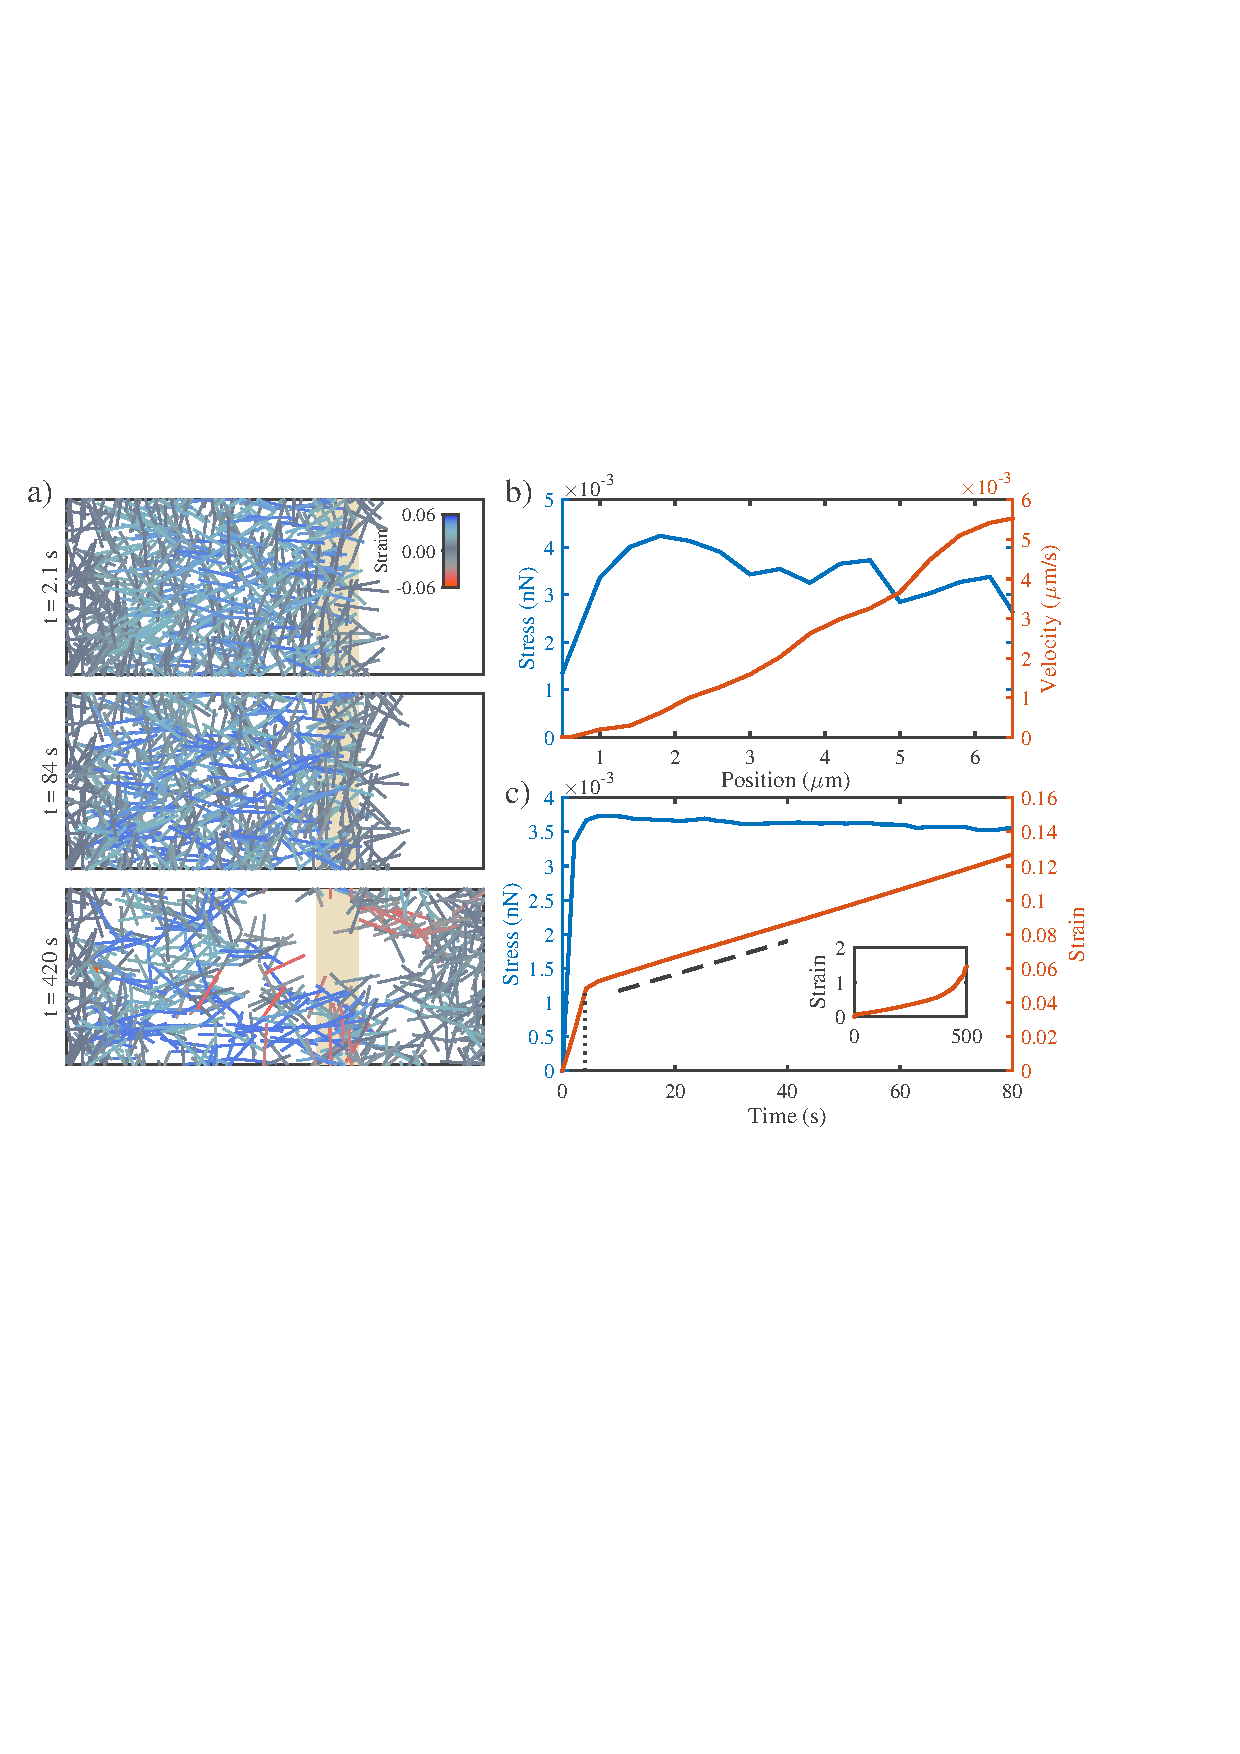
\includegraphics[width=\hsize]{figures/figure3a}
\caption{\label{fig:passive_ex}  Networks with passive cross-links and no filament turnover undergo three stages of deformation in response to an extensional force.   \textbf{a)} Three successive time points from a simulation of a $4\times10\: \mu m$ network deforming under an applied extensional stress of 0.005 $nN/\mu m$ (stress is applied to filaments in the region indicated by the tan bar). In this and all subsequent figures, filaments are color-coded with respect state of stress (blue = tension, red = compression).  Network parameters: $L=1\: \mu m$, $l_c=0.3\: \mu m$, $\xi=100\: nN\cdot s/\mu m$. \textbf{b)} Mean filament stress and velocity profiles for the  network in (a) at t=88s. Note that the stress is nearly constant and the velocity is nearly linear as predicted for a viscous fluid under extension.  \textbf{c)} Plots of the mean stress and strain vs time for the simulation in (a), illustrating the three stages of deformation: (i) A fast initial phase accompanies rapid buildup of internal network stress; (ii) after a characteristic time $\tau_c$ s (indicated by vertical dotted line) the network deforms like a material with a constant effective viscosity, $\eta_c$, as indicated by the slope of the dashed line; (iii) at long times, the strain accelerates (see inset) as the network undergoes strain thinning and eventually tears. }
\end{figure}

% Viscosity and timescale parameter dependence
\paragraph{Network architecture sets the rate and timescales of deformation.}  To better understand how network architecture and cross-link dynamics control effective viscosity and the timescale for transition to viscous behavior, we systematically varied network parameters (see Table \nameref{S1_Table}), and measured the elastic modulus, $G_0$, effective viscosity, $\eta_c$, and transition time, $\tau_c$, in response to a fixed external stress. We observed the transition from a viscoelastic to an effectively viscous phase for the entire range of parameters that we sampled.  The elastic limit that we observe during the viscoelastic phase agreed closely with the closed form solution for the elastic modulus  $G_0 \sim \mu/l_c$ predicted by a previous model \cite{theo_hlm} for networks of semi-flexible filaments with irreversible cross-links (\nameref{fig:passive_supp}). A simple theoretical analysis (shown in \nameref{S1_Text}) predicts that in the effectively viscous phase, the effective viscosity should be proportional to the effective cross-link drag coefficient and to the square of the number of cross-links per filament, with a constant of proportionality $\pi/4$. As shown in Figure \ref{fig:passive_form}a, our simulations agree well with this prediction for a large range of network parameters. For many linear viscoelastic materials, the ratio of the elastic modulus, $G_0$, to the viscosity $\eta_c$, is a general indicator of the transition timescale from elastic to viscous behavior\cite{mccrum1997principles}. Using our approximations of the elastic modulus and viscosity, we predict a crossover time, $\tau_c \approx L^2\xi/l_c\mu$. By measuring the time at which the strain rate became nearly constant we obtained an estimate of this time for a wide variety of simulation parameters. As shown in Figure \ref{fig:passive_form}b, our approximation is in good agreement with the observed transition time, indicating that the passive responses of our simulated networks are well represented by effectively linear bulk properties.


\begin{figure}[h!]
\centering
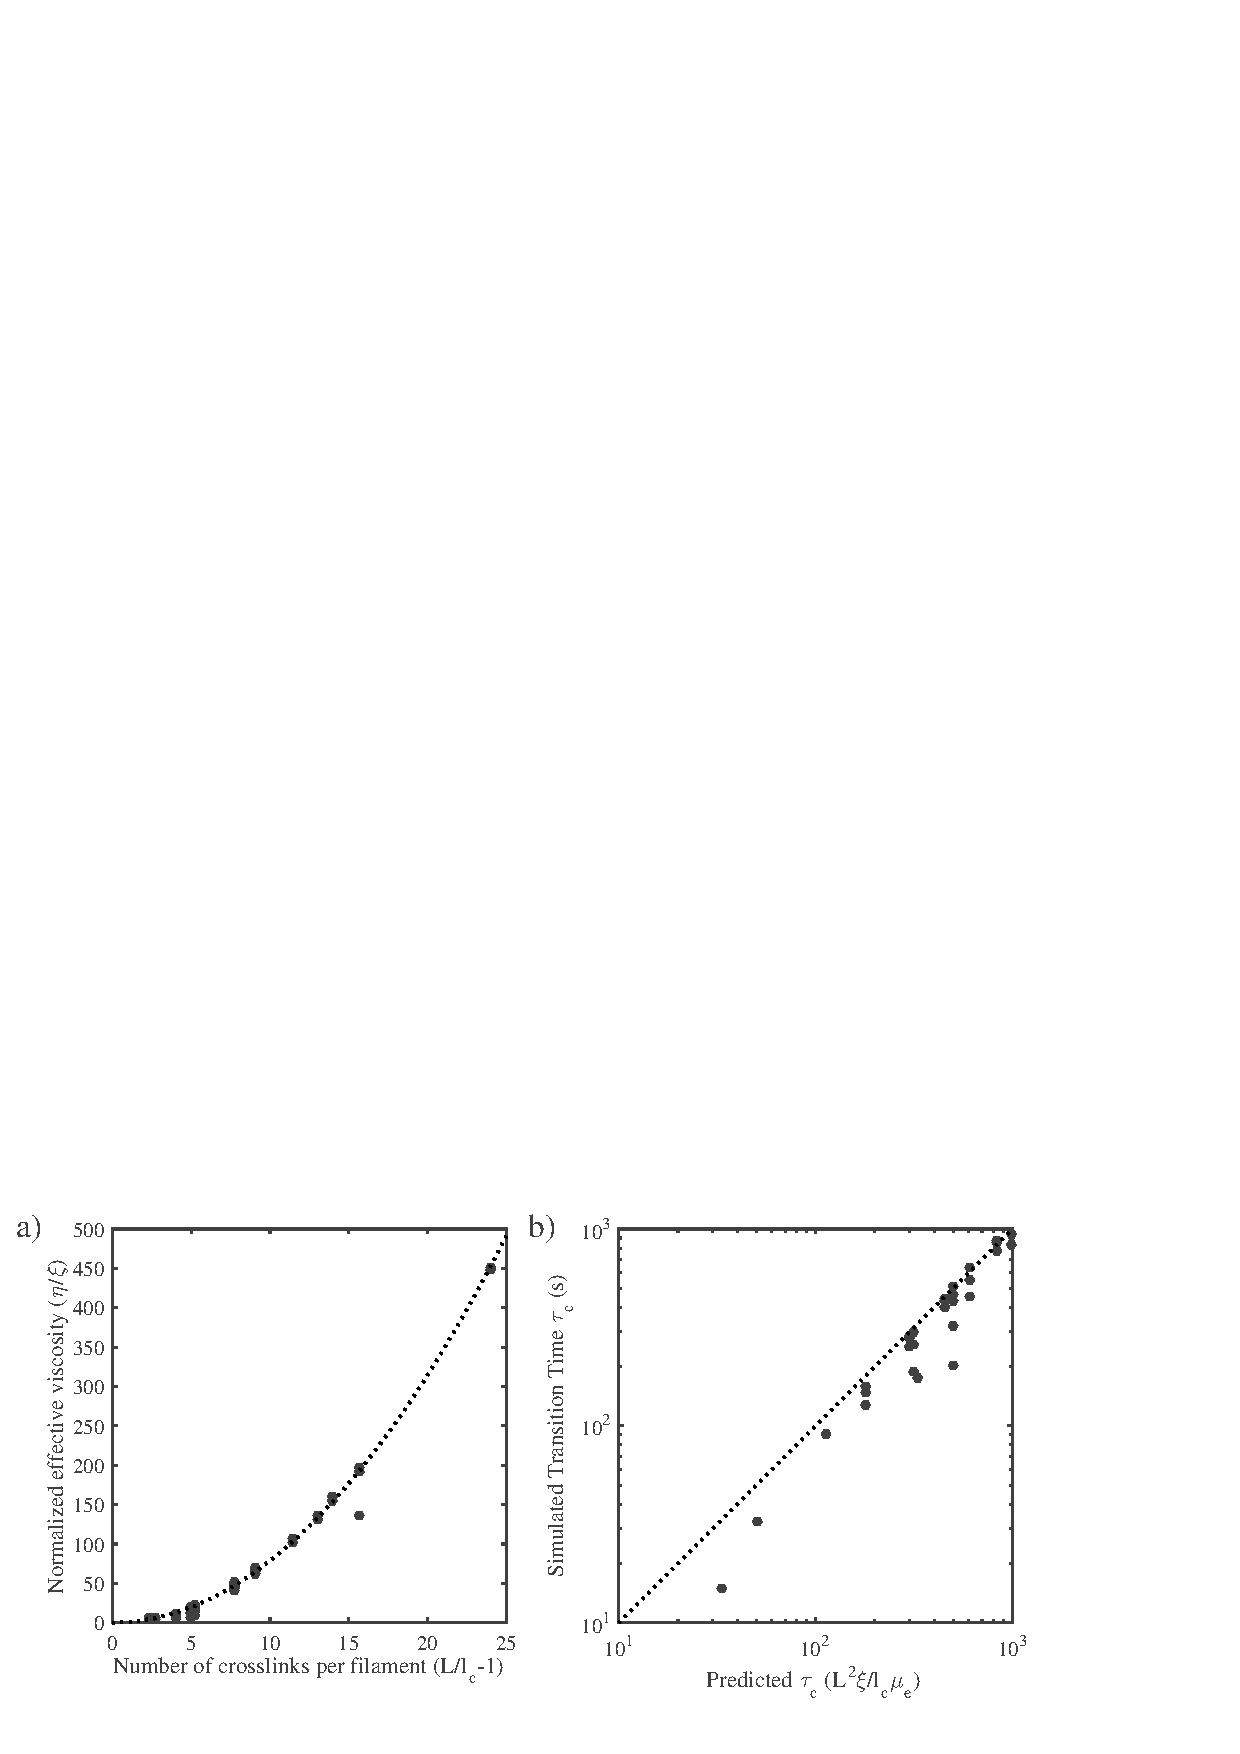
\includegraphics[width=\hsize]{figures/figure3b}
\caption{\label{fig:passive_form} Network architecture sets the rate and timescales of deformation. \textbf{a)} The effective viscosity depends on the drag coefficient and the density of the network. Data points are the normalized effective viscosity from simulations (effective viscosity measured in fluid phase divided by the cross link friction coefficient) vs the number of cross links per filament $(L/l_c - 1)$.  Dotted line indicates the relationship predicted by a simple theory, $\eta_c = \xi(L/l_c-1)^2$ \textbf{b)} The transition to viscous behavior occurs at a characteristic time, $\tau_c$, that is set by the ratio of the elastic modulus predicted in \cite{theo_hlm} (i.e. $G_0 \approx \mu/l_c$) to the effective viscosity, $\eta_c$.  }
\end{figure}


% Passive Recycling
\paragraph{Filament recycling rescues network tearing and modulates effective viscosity.} 
 
\begin{figure}[h!]
	\centering
	\includegraphics[width=\hsize]{figures/figure5a}
	\caption{\label{fig:passive_rec}  Filament recycling modulates effective viscosity in two regimes. \textbf{a)} Examples of $20 \times 12 \mu m$ network under 0.001 $nN/\mu m$ extensional stress with recycling ($\tau_r=10 s$) and without, ($\tau_r=\infty$).  Both images are taken when the patches had reached a net strain of 0.4.  The network with recycling doesn't appear to change shape because its components have been recycled to remain in the original domain.  Network parameters: $L=3\: \mu m$, $l_c=0.5\: \mu m$, $\xi=10\: nN\cdot s/\mu m$. \textbf{b)} Strains curves for identical networks with varying levels of filament recycling.  Network parameters: $L=3\: \mu m$, $l_c=0.5\: \mu m$, $\xi=10\: nN\cdot s/\mu m$. \textbf{c)}  Plotting the effective viscosity derived from the slopes of the lines in panel a. The values have been normalized to the predicted effective viscosity. \textbf{d)} Normalized effective viscosities as a function of the normalized recycling time. When the recycling timescale is significantly less than the passive relaxation timescale, the viscosity of the network becomes dependent on recycling time.}
\end{figure}

To explore how filament recycling shapes the passive network response to an applied force, we ran a series of simulations with identical filament lengths and network densities and cross-link drag coefficients, while varying the filament recycling time $\tau_r=1/k_{diss}$. Figure \ref{fig:passive_rec}a illustrates the results for a particular set of network parameters. In the absence of filament recycling, strain thinning and network tearing lead to a rapid increase in strain rate above a critical strain of $\sim40\%$. 

Progressively decreasing the filament recycling time led to a progressive increase in the rate of network deformation during the effectively viscous phase and an increase in the critical strain at which the network began to tear. Below a critical recycling time ($\tau_{crit}$), the network could sustain effectively viscous deformation indefinitely, as shown by the lack of strain thinning in the strain profiles of Figure\ref{fig:passive_rec}b. Intuitively, steady state deformation is achieved when the rate of filament depletion by strain thinning is balanced by a sufficiently high rate of filament recycling (i.e. a sufficiently low recycling time).  To determine the critical recycling time, we write an equation for the rate of change in filament density $\rho$, as a function of filament recycling ($k_{app}-k_{diss}\rho$) and strain thinning ($-\dot{\gamma}\rho$).
These terms can be rewritten to give the following 

\begin{equation}
\frac{d \rho}{dt} = \frac{\rho_0-\rho}{\tau_r}  - \frac{\sigma}{\eta_c(\rho)} \rho
\end{equation}

where $k_{diss}$  has been replaced by $1/\tau_r$, and $\rho_0 = k_{app}\tau_r$, and $\dot{\gamma}$ has been replaced by $\sigma/\eta_c$.  For our networks, the effective viscosity, $\eta_c$, is dependent on the filament density (through $l_c$) so this dependence must be included. Solving this equation for its steady states, and replacing the initial density, $\rho_0$, with the length density approximation, $1/l_c$, we find that a steady state density only exists under the condition $\tau_r < \tau_{crit}=\eta_c/4\sigma$.  

Reducing recycling time, $\tau_r$, below $\tau_{crit}$ produced different effects on steady state deformation rates depending on the relative values of $\tau_r$ and $\tau_c$, the characteristic time for transition to effectively viscous deformation in the absence of recycling. For $\tau_r > \tau_c$, the effective viscosity remained $\sim$constant with decreasing $\tau_r$; for $\tau_r < \tau_c$, effective viscosity decreased linearly with decreasing $\tau_r$.  The intuitive explanation for this is as follows: For $\tau_r > \tau_c$, the deformation rate is dominated by cross-link resistance to sliding of strained filaments. For $\tau_r < \tau_c$, the deformation rate is limited by the level of elastic stress on partially strained filaments; By replacing partially strained with unstrained filaments, the network is able to tune the mean level of stress and thus the deformation rate.


To confirm this relationship more generally, we allowed filament lengths, network density and cross link friction to vary more widely, and we measured the network deformation rates while varying filament recycling times (Figure \ref{fig:passive_rec}a,b). We then plotted the normalized effective viscosity (ratio of effective viscosity with recycling to effective viscosity without recycling, $\eta_c$) vs a normalized recycling rate (recycling time scaled by $\tau_c$). Indeed, we found that the normalized effective viscosity measured during steady state flow begins to decrease when the recycling time falls below $\tau_c$ and below this value the effective viscosity falls off linearly with recycling time to minimal values (Figure \ref{fig:passive_rec}c). 

To describe this we introduce (based on linear viscoelastic models of \cite{mccrum1997principles}) an effective recycling viscosity, $\eta_r$, which can be tuned between the $\tau_r$ dependent and independent regimes, depending on the value of the recycling timescale.



\begin{equation}
\label{eqn:simple_eta}
\eta_r = \frac{\eta_c}{1+\tau_c/\tau_r}  
\end{equation}

For $\tau_r\gg\tau_c$, this simplifies to $\eta_r\approx\eta_c$, while for  $\tau_r\ll\tau_c$, this simplifies to $\eta_r\sim\tau_r/\tau_c$, which matches qualitatively with our estimate as found in Figure \ref{fig:passive_rec}d for a large range of parameters. This model presents a simple quantitative description of our simulation data.



%Discuss
In summary, we find that tuning recycling times above a critical value $\tau_{crit}$, allows networks to undergo continuous viscous deformation, for long times, without tearing, for a wide range of different effective viscosities and deformation rates. For $\tau_r < tau_{crit}$, modulating filament recycling times can tune the network between two regimes. For $\tau_r > \tau_c$, the deformation is limited by effective cross-link friction, the effective viscosity depends on the strength of inter-filament cross-linking and the network's architecture, and is relatively insensitive to changes in recycling rate. For $\tau_r < \tau_c$, the deformation is governed by the buildup of elastic stress on network filaments, and effective viscosity becomes strongly dependent on recycling time. 

These findings are in agreement with previous simulations on effective viscosity in cross-linked networks. A previous analysis \cite{Kim2014526} looked at the effect of a different form of filament turnover in networks with irreversible cross-linking. The authors also showed two regimes of deformation: one in which network deformation was linearly viscous and tuned by the turnover rate, and one where the creep rate was set purely by the turnover rate independent of applied force.  Although the implementation is different, the two regimes observed in our model are in qualitative agreement and arise from similar microscopic origins. Specifically, the short recycling time regime, where the mechanics are governed by filament extension, is directly equivalent in both models.  For this regime, our model is able to give a theoretical description of the effective viscosity found in \cite{Kim2014526}.  For the opposite regime of long recycling times, the models have a distinct difference.  For the model of \cite{Kim2014526} there was no cross-link unbinding so without of filament turnover, the network would not deform beyond its elastic limit.  In contrast, our simulations always require non-zero cross-link slip so there is always some viscous network deformation.  Therefore, in the regime of long recycling times our model approaches the limit of cross-link dominated viscosity whereas the model of \cite{Kim2014526} approached an infinite viscosity limit.






% ACTIVE SECTION
\subsection*{Filament recycling allows persistent stress buildup in active networks}

\paragraph{In the absence of filament recycling, active networks with free boundaries contract and then stall against passive resistance to network compression.}

\begin{figure}[h!]
	\centering
	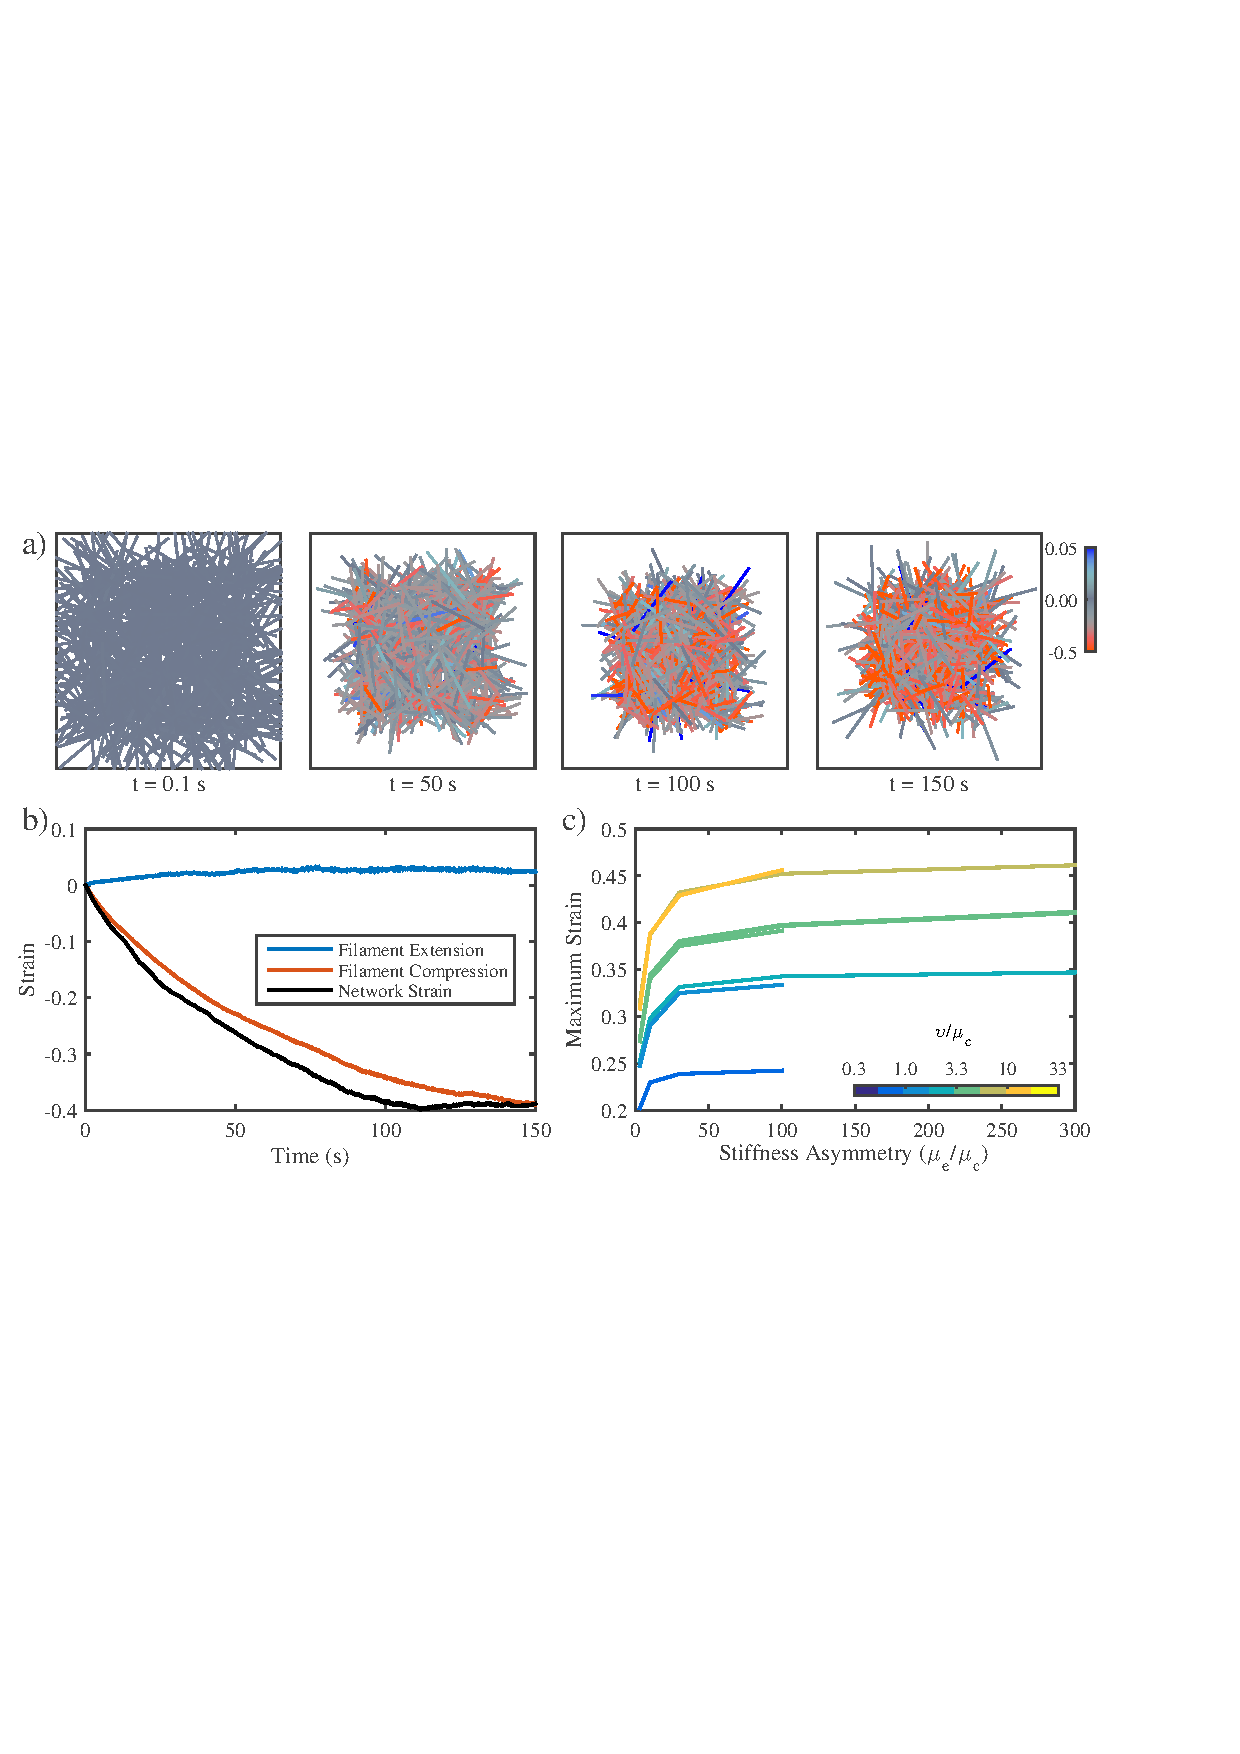
\includegraphics[width=\hsize]{figures/figure4a}
	\caption{\label{fig:active_con} In the absence of filament recycling, active networks with free boundaries contract and then stall against passive resistance to network compression. \textbf{a)}  Example of an active network contracting. Note the buildup of compressive stress as contraction approaches stall between 100 s and 150 s.  Network parameters: $L=5\: \mu m$, $l_c=0.3\: \mu m$, $\xi=100\: nN\cdot s/\mu m$, $\upsilon=0.1\: nN$.  \textbf{b)} Plots showing time evolution of total network strain and  the average extensional (blue) or compressive (red) strain on individual filaments.   \textbf{c)} The network's ability to deform requires asymmetric filament compliance.  Total network strain also increases with the applied myosin force $\upsilon$. Note that the extent of contraction approaches an asymptotic limit as the stiffness asymmetry approaches a ratio of $\sim 100$.}
\end{figure}

Previous theoretical and experimental studies\cite{1367-2630-14-3-033037,rheo_2D1,rheo_active} identified asymmetric filament compliance and dispersion in motor force  as minimal requirements for contraction of disordered networks.To test if our simple implementation of these two requirements (see above) was sufficient to produce macroscopic contraction, we simulated active networks that were unconstrained by external attachments.  Turning on motor activity in an initially unstrained network at $t=0$ produced a rapid initial contraction, followed by a progressive buildup of elastic stress due to compression of individual filaments and an $\sim$exponential approach to stall. On a longer timescale, polarity sorting of individual filaments, as previously described \cite{Ndlec:1997aa,Surrey1167} rearranged the entire network, undoing the initial contraction (see \nameref{active_con_video}).  


We focus here on the contraction phase. During the rapid initial contraction, bulk network strain matched closely the mean compressive strain on individual filaments Figure \ref{fig:active_con}b, Thus  confirming that the origin of bulk contraction in our simulations is filament ?buckling? due to asymmetric filament compliance, as predicted by \cite{1367-2630-14-3-033037,PhysRevX.4.041002} and observed experimentally\cite{rheo_2D1}. Contraction only occurred when the fractional motor activity $0<\phi<1$ (i.e. the fraction of filament intersections with active motors) was less than one, confirming the requirement for dispersion of motor activity (see \nameref{fig:active_supp}) Thus our model effectively captures a minimal mechanism for bulk contractility in disordered networks through asymmetric filament compliance and dispersion of motor activity.

We also determined how microscale parameters shape the rate and final extent of network contraction. Consistent with the idea that contraction stalls when the elastic resistance to filament compression balances the contractile stress., the final extent of contraction increased sharply with motor activity ($\upsilon$) and with the asymmetry in filament stiffness (i.e. the ratio of the extensional and compressive stiffnesses $\mu_e/\mu_c$, Figure \ref{fig:active_con}c,  The time to stall, $\tau_m$, scaled as $L\xi/\upsilon$ (see \nameref{fig:active_supp}b), although the origins of this scaling relationship remain unclear. 


\paragraph{Active networks can only exert a transient force against a fixed boundary in the absence of filament recycling.}

\begin{figure}[h!]
	\centering
	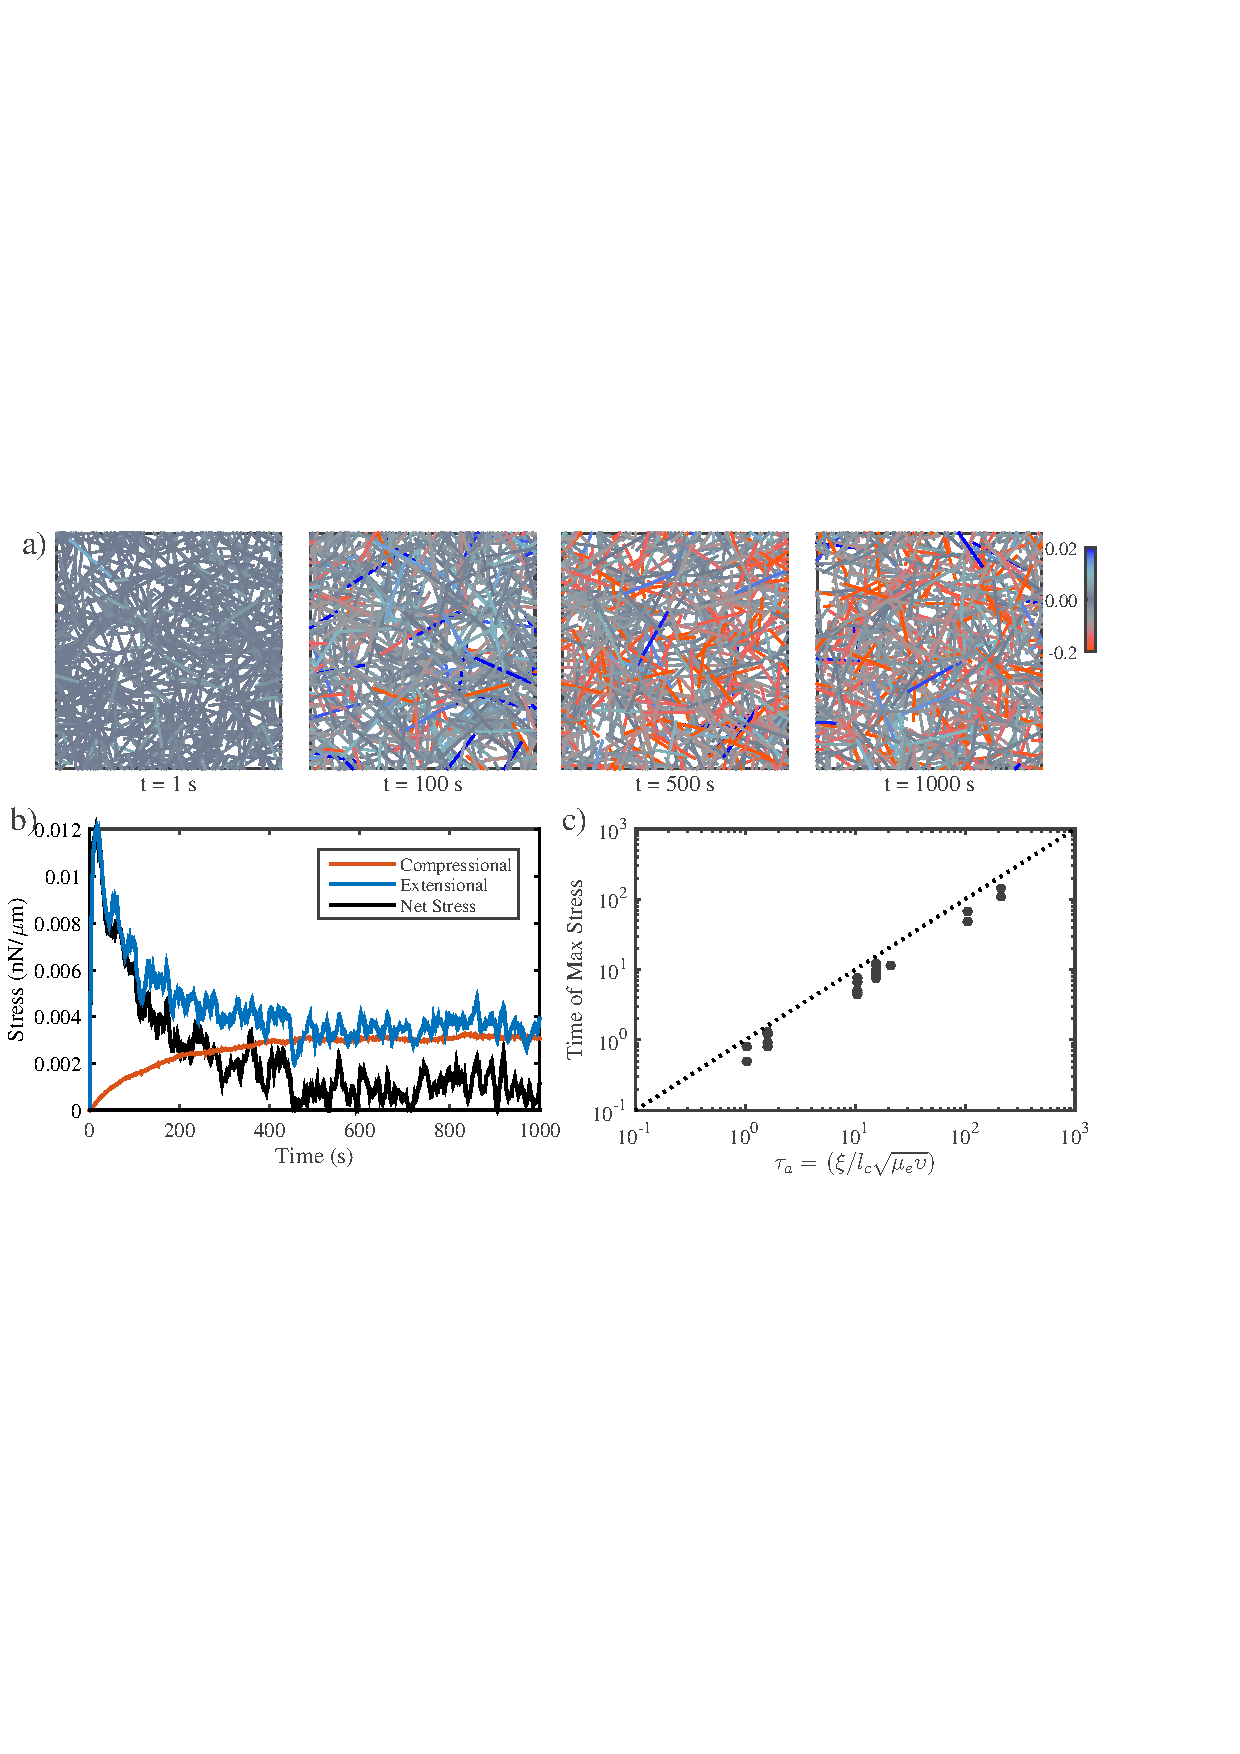
\includegraphics[width=\hsize]{figures/figure4b}
	\caption{\label{fig:active_str} In the absence of filament recycling, active networks can only exert a transient force against a fixed boundary.  \textbf{a)} Simulation of an active network with fixed boundaries illustrating progressive buildup of internal stress through local filament rearrangement and deformation. Note the progressive buildup of compressive stress on individual filaments. Network parameters: $L=5\: \mu m$, $l_c=0.3\: \mu m$, $\xi=100\: nN\cdot s/\mu m$, $\upsilon=0.1\: nN$.  \textbf{b)} Plots of total network stress and the average extensional (blue) and compressive (red) stress on individual filaments for the simulation shown in (a). Rapid buildup of extensional stress allows the network transiently to exert force on its boundary, but this force is dissipated at longer times as   as internal extensional and compressive stresses become balanced. \textbf{c}. Measurement and prediction of the characteristic time ($\tau_a$) at which the maximum stress is achieved. }
\end{figure}

The previous results reveal internal limits on the contraction of networks with free boundaries.  However networks typically build force and contract against an external resistance.  Therefore, we analyzed the buildup and maintenance of contractile stress in active networks contracting against a rigid boundary. We simulated active networks contracting from an initially unstressed state against a fixed boundary Figure \ref{fig:active_str}a, and  quantified the time evolution of mean extensional (blue), compressional (red) and total (black) stress on network filaments \ref{fig:active_str}b. We observed the same qualitative behavior for all network parameters examined: Total stress built rapidly to a peak value $\sigma_a$, and then decayed back to zero again.  The initial rise in total stress was driven by a  rapid buildup of extensional stress, while the decay was caused by a slower dissipation of extensional stress and a comparably slow buildup of compressional stress.  

Sampling these dynamics over a large range of network parameters, we found that the peak stress occurred at a characteristic time, $\tau_a=\xi/l_c\sqrt{\mu\upsilon}$, as shown in Figure \ref{fig:active_str}c. 
{\em Need to say something here about the slower timescale of stress dissipation.  I understand that you have not yet found a scaling relationship for this one.  But it would be very nice, even if you can?t find such a relationship, to have a comparison between  the timescale to reach stall for the freely contracting network and the time to dissipate contractile stress in the pinned case. I.e. is one always bigger than the other for a particular choice of parameters? }

Thus, in the absence of filament turnover, local filament deformation and rearrangement leads to a gradual dissipation of network stress that limits the ability of a networkexert sustained force on its boundaries. 


\paragraph{Filament recycling allows networks to exert sustained stress on a fixed boundary.}

\begin{figure}[h!]
	\centering
	\includegraphics[width=\hsize]{figures/figure5b}
	\caption{\label{fig:active_rec} Filament recycling allows network to exert sustained stress on a fixed boundary. \textbf{a)} Snapshots from simulations of active networks with fixed boundaries for different timescales of filament recycling.  Network parameters are the same as in Figure 6. Note that significant remodeling occurs for longer recycling times. \textbf{b)} Plots of net stress exerted by the network on its boundaries for different recycling times; for long-lived filaments, stress is built rapidly, but then dissipates. Increasing filament turnover rates reduces stress dissipation by recycling compressed filaments; however, very short recycling times prevent any stress from being built up in the first place. \textbf{c)} Plotting the steady state stress derived from the long term stress values of the stress in panel b.  \textbf{d)} Normalized steady state stress as a function of normalized recycling time. The steady state stress is set by the timescale at which the network strain is refreshed relative to the timescale at which the max stress is reached. The values have been normalized to the predicted effective viscosity, $\eta_c$ in the absence of recycling.}
\end{figure}

To explore how this limitation could be relieved by filament recycling, we considered an active network contracting against a fixed boundary, using the same parameters as in Figure \ref{fig:active_str}, and systematically varied filament recycling rates. Adding filament recycling produced two general effects: First, as for the passive case, filament recycling could prevent catastrophic tearing by continuously repairing local structural heterogeneities, and by steadily opposing the effects of local strain thinning (see \nameref{fig:tear_supp}). Second, we found that filament recycling resulted in biphasic modulation of the level of steady state stress.

 For the same network parameters as in Figure \ref{fig:active_rec}a and slow filament recycling ($\tau_r = 1000 s$), the network stress peaked rapidly, but then relaxed to a lower value that persisted for times much longer than $\tau_a$. Decreasing recycling time produced a sharp increase in the steady state stress, although the steady state stress remained lower than its peak value.  However, further decreases in recycling time lead to decreases in the steady state stress as well as sharp decreases in the peak stress. Intuitively, this bimodal dependence of steady state stress on recycling rates emerges from continuous replacement of strained with unstrained filaments, combined with the different timescales for buildup of extensional vs compressive filament stress (Figure \ref{fig:active_rec}b). Because extensional stress builds more rapidly than compressive stress, lowering the recycling time $\tau_c$ should increase net stress until $\tau_c$ is approximately equal to $\tau_a$, the time required to build peak stress from an initially unstressed state. For shorter recycling times, the average filament will not have time to build maximum extensional stress before turning over, and thus the steady state stress should decrease with further decreases in $\tau_c$. Plotting normalized steady state stress (steady state stress/peak stress) vs normalized recycling time ($\tau_c$ /$\tau_a$) confirms that this biphasic dependence of steady state stress on recycling times holds for a large range of sampled values for network parameters \ref{fig:active_rec}d.


In the same manner as for the equation of passive response (i.e. Equation \ref{eqn:simple_eta}), we can approximate the dependence of the steady state stress on the filament recycling rate using a simple equation. 

\begin{equation}
\label{eqn:simple_sigma}
\sigma_{ss} = \frac{\sigma_{peak}}{(\tau_r/\tau_a)^n+\tau_a/\tau_r}  
\end{equation}

For $\tau_r\gg\tau_a$, this simplifies to $\sigma_{ss}\sim(\tau_a/\tau_r)^n$, while for $\tau_r\ll\tau_a$, this simplifies to $\sigma_{ss}\sim\tau_r/\tau_a$. What sets the scaling $n$ remains unclear, and this scaling does not appear to be consistent across all simulation setups (Figure \ref{fig:active_rec}d). However, equation \ref{eqn:simple_sigma} still captures a qualitatively correct description of steady state stress in our simulation data.


We repeated the single domain (passive or active) simulations while varying all of our networks microscopic parameters.   By exploring the effect of these parameters on the output variables we were able to determine the general form of the dependence. In Figure \ref{fig:passive_rec}d, we illustrate the data collapse of all our simulation results (see \nameref{S1_Table} for details of parameter exploration).  Interestingly, both the viscosity (in Figure \ref{fig:passive_rec}d) and stress (in Figure \ref{fig:active_rec}d) show changes in behaviors on either side of their respective governing timescales ($\tau_c$ for viscosity and $\tau_a$ for active stress).  Effective viscosity was found to be independent of recycling time until recycling time became of the same order as the elastic to viscous crossover timescale, at which point it decreased with decreasing recycling time.  Similarly, the steady state stress increases with increasing recycling time until it reaches the point of peak stress buildup.  From that point it decreases with increasing recycling time.  Taken together, these effects would suggest a simple predicted flow for a given network setup. 







% COMBINED SECTION
\subsection*{Filament recycling tunes the balance between active stress buildup and viscous stress relaxation to generate flows}

Thus far, we have characterized how filament recycling tunes effective viscosity during passive deformation in response to an externally applied stress the steady state stress produced by an active network against an external resistance.  We next sought to characterize how filament recycling tunes steady flows produced by gradients of motor activity in a region of high motor activity contracts against the passive resistance of a neighboring region with low motor activity.  

\paragraph{Filament recycling allows sustained flows in networks with non-isotropic activity.}

\begin{figure}[h!]
	\centering
	\includegraphics[width=\hsize]{figures/figure6a}
	\caption{\label{fig:flow_ex}  Filament recycling allows sustained flows in networks with non-isotropic activity. \textbf{a)} Example simulations of non-isotropic networks with long ($\tau_r=1000$) and short ($\tau_r=33$) recycling timescales. In these networks the left half of the network is passive while the right half is active.  Network parameters are same as in Figures \ref{fig:active_str} and \ref{fig:active_rec}. Importantly, in all simulations $\tau_a<\tau_c$. \textbf{b)} Graph of strain for identical networks with varying recycling timescales.  With long recycling times, the network stalls; reducing the recycling timescale allows the network to persist in its deformation.  However, for the shortest recycling timescales, the steady state strain appears to approach an asymptotic limit.  \textbf{c)} Graph of network long-term strain rate as a function of recycling timescale for simulations in a) and b). \textbf{d)} Graph of network long-term strain rate as a function of recycling timescale across a wide range of parameter space.  Note that networks only begin to maintain long-term flows when the recycling time is less than $100\tau_a$. }
\end{figure}

We imposed a continuously asymmetric distribution of motor activity on an initially uniformly dense network of passively cross-linked filaments by allowing a fraction of cross links to be active only in the right half of the simulation domain. Then we examined the time-dependent deformation of the network for a range of different filament recycling times Figure \ref{fig:flow_ex}a. We observed a sharp dependence of steady flow on filament recycling rate Figure \ref{fig:flow_ex}b,c. For very longer recycling times, ($\tau_r=1000 s$, dark blue line), there was a rapid initial deformation (contraction of the active domain and dilation of the passive domain), followed by a slow approach to a steady state flow characterized by slow contraction of the right half-domain and a matching dilation of the left half-domain (see \nameref{fig:combo_prof}).  However, with decreasing filament recycling times, we found the network was able to sustain its deformation and that the long term strain rate rose toward an asymptotic limit (Figure \ref{fig:flow_ex}c).  We repeated these measurements for more network parameters and found that at the shortest recycling timescales measured, we still saw the effective viscosity remaining relatively high, indicating that for sufficiently short recycling times the effective viscosity may approach an asymptotic flow rate (Figure \ref{fig:flow_ex}d).







\paragraph{Filament recycling tunes the magnitudes of both effective viscosity and steady state stress.}  


\begin{figure}[h!]
	\centering
	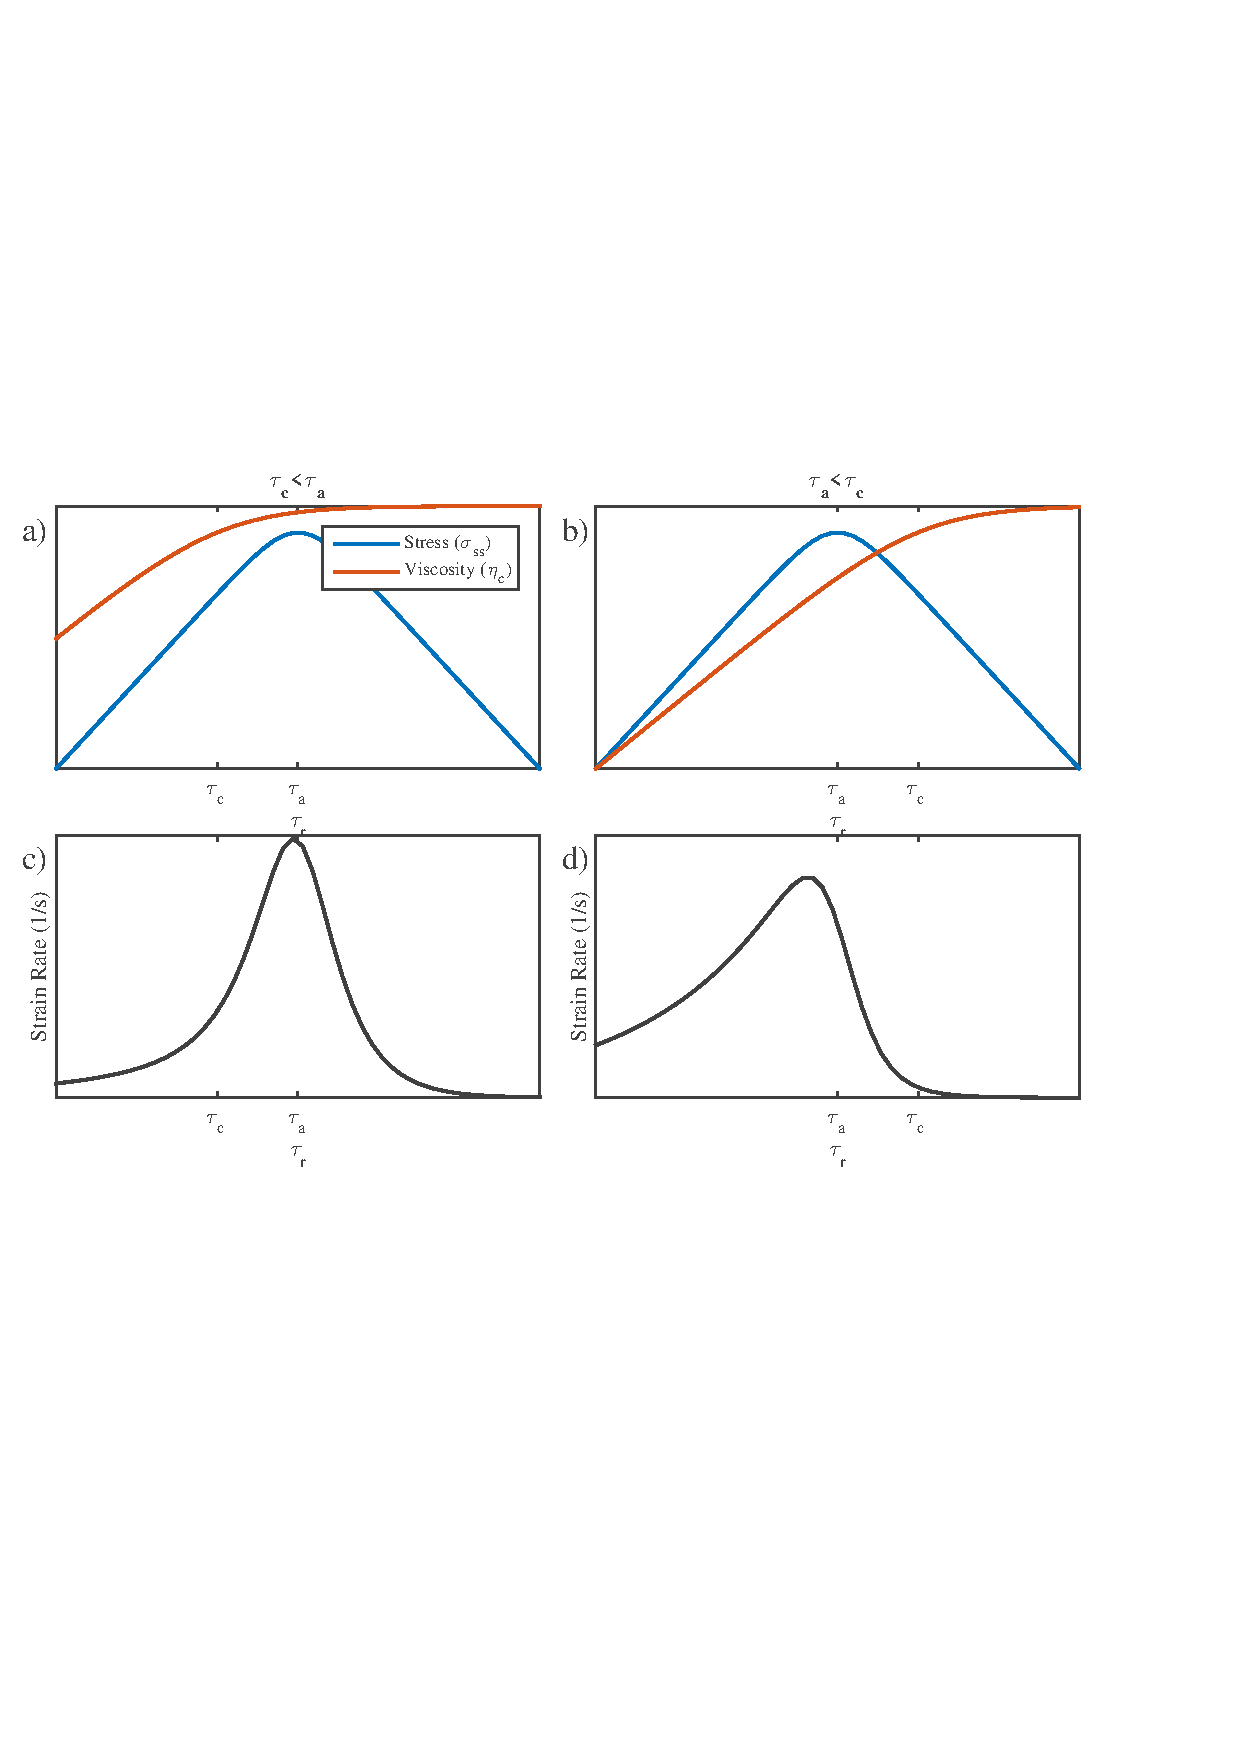
\includegraphics[width=\hsize]{figures/figure_theor}
	\caption{\label{fig:flow_theo}  Filament recycling tunes the magnitudes of both effective viscosity and steady state stress. \textbf{a)}  Dependence of steady state stress and effective viscosity on recycling time $\tau_r$ under the condition $\tau_c<\tau_a$. \textbf{b)} Same as a), but for the case where $\tau_a<\tau_c$.  \textbf{c,d)} Resulting strain rates for network as a function of recycling time $\tau_r$ for the regimes in panels a and b..  }
\end{figure}

This dependence of steady state deformation (flow) rate on filament recycling times can be understood in terms of our previous findings.  During steady state flow, active contraction of the right half-domain is limited both by internal resistance to compression of filaments within the right half-domain (Figure 5), and by passive resistance of the left-half domain (Figure 4).  

Monitoring these two forms of resistance as a function of filament recycling time for the simulations in Figure 8, we see that resistance to compression of filaments in the right half domain makes a significant contribution only for very low recycling rates.  This is again because compressional resistance on filaments in the contracting right half domain takes longer to build than extensional resistance on filaments in the dilating right half-domain. As a consequence, except for very low recycling rates,  steady state deformation is governed by an equation of the form:

\begin{equation}
\label{eqn:simple_sigma}
\dot{\gamma} = \frac{\sigma_{ss}}{\eta_r}  
\end{equation}

where $\sigma_{ss}$ is the active stress generated by the right half-domain (less the internal resistance to filament compression), $\eta_r$ is the effective viscosity of the left half domain and strain rate is measured in the left half-domain.  Therefore, we can understand the dependence of network flow (i.e. strain rate) on filament recycling time $\tau_r$ in terms of the previously characterized dependencies of effective viscosity and steady state stress on $\tau_r$ (Figures \ref{fig:passive_rec}d and \ref{fig:active_rec}d). In particular, recall that there is a transition in the dependence of $\eta_r$ on $\tau_r$ at the characteristic time $\tau_c$, and a transition in the dependence of sigma on $\tau_r$ at the characteristic time $\tau_a$.  Thus, as shown in Figure \ref{fig:flow_theo},  there are two qualitatively distinct cases for the dependence of strain rate on $\tau_r$, depending on the relative magnitudes of $\tau_a$ and $\tau_c$.  For both cases, we expect an increase in strain rate with filament recycling at long recycling times (where effective viscosity is insensitive to strain rate)  and approach to an asymptotic strain rate at low recycling times, where both $\eta_r$ and $\sigma_{ss}$ fall off approximately linearly. For $\tau_a < \tau_c$, we predict a peak strain rate at intermediate recycling times, whereas for $\tau_a > \tau_c$, we expect a simpler monotonic approach to maximum strain rate at low recycling times.  As shown in Figure \ref{fig:flow_theo}d, for the range of network parameters we sampled, the dependence of strain rate on $\tau_r$ is monotonic and approaches an asymptote at low recycling times (i.e. high recycling rates).  This is to be expected because all the parameter values sampled (selected for physiological relevance) satisfied the condition $\tau_a > \tau_c$.



\paragraph{Filament recycling influences architectural control of flow rate.}

\begin{figure}[h!]
	\centering
	\includegraphics[width=\hsize]{figures/figure6b}
	\caption{\label{fig:flow_form}  Filament recycling influences architectural control of flow rate. \textbf{a)}  For a fixed filament recycling time, filament length tuned network deformation rate.  \textbf{b)} Recycling rate is independent of cross-link spacing in this parameter space.}
\end{figure}

Finally, we examined how steady state flow depends on other network parameters when filament recycling rates are held constant.   Interestingly, we found that flow rates are largely insensitive to cross link density ($l_c$) but vary inversely with filament length. Thus, in this region of parameter space, steady state flows may be buffered intrinsically against some forms of variation in network architecture.










%Conclusion
\section*{Conclusion}
Our work aimed to create a simulation framework that would allow us to analyze the origins of macroscopic flow in terms of a handful of physiologically relevant microscopic parameters.  Toward this aim we developed a minimalist model of a 2D filament network and analyzed the network's reaction to a variety of situations.  We found mathematical relationships that determined both the passive effective viscosity and the active stress generation of networks with and without recycling.  From these relationships we were able to make predictions about the rates of network flow in non-isotropic networks mimicking those found in polarized eukaryotic actomyosin cortices.  

Importantly, our work brings a theoretical understanding to the importance of actomyosin turnover in producing and maintaining long-term large scale flows.  We propose the concept of "filament recycling" to refer to the multitude of biochemical interactions which can give rise to the piece by piece architectural resetting of filament networks.  We believe that our analysis of networks in the presence of this filament recycling will be useful in further developing the qualitative and quantitative understanding the deformation of these complex networks.

\section*{Supporting Information}

% Include only the SI item label in the subsection heading. Use the \nameref{label} command to cite SI items in the text.
\paragraph*{S1 Text.}
\label{S1_Text}
{\bf Bold the title sentence.} Add descriptive text after the title of the item (optional).

\paragraph*{S1 Fig.}
\label{S1_Fig}
{\bf Bold the title sentence.} Add descriptive text after the title of the item (optional).

\paragraph*{S2 Fig.}
\label{fig:passive_supp}
{\bf  Mechanical properties of passive networks.}  \textbf{a)} Elastic modulus of networks.  Our measurements closely match prediction of $G_0\sim\mu/l_c$.  \textbf{b)}  Placeholder for inevitably another figure relevant to passive properties..

\paragraph*{S3 Fig.}
\label{fig:tear_supp}
{\bf Mechanical properties of active networks } Add descriptive text after the title of the item (optional).

\paragraph*{S4 Fig.}
\label{fig:active_supp}
{\bf Mechanical properties of active networks } Add descriptive text after the title of the item (optional).

\paragraph*{S6 Fig.}
\label{fig:combo_prof}
{\bf Spatial velocity profile of networks containing passive and active domains.} 

\paragraph*{S1 Table.}
\label{S1_Table}
{\bf Parameter values.}  List of parameter values used for each set of experiments.

\paragraph*{S1 Video.}
\label{passive_ex_video}
{\bf Extensional strain in passive networks.}  Movie of simulation setup shown in Figure \ref{fig:passive_ex}

\paragraph*{S2 Video.}
\label{active_con_video}
{\bf Active networks contracting with free boundaries.}  Movie of simulation setup shown in Figure \ref{fig:active_con}

\section*{Acknowledgments}
We would like to thank Shiladitya Banerjee and Patrick McCall for stimulating discussions.

\nolinenumbers

%\section*{References}
% Compile your BiBTeX database using our plos2015.bst
% style file and paste the contents of your .bbl file
% here.
% 
\bibliographystyle{plos2015}
\bibliography{slippage,active}



\end{document}

